\section{Registered study on recorded robot video}
\label{app:real-video}
\IfFileExists{tables/real_video_results.tex}{
\noindent\textbf{Status: complete prespecified real-data comparison.}
}{\noindent\textbf{Status: data audit complete; model comparisons pending.}}
This additional study evaluates forecasting on real robot recordings from
DROID~\citep{khazatsky2024droid}. It complements the simulator experiments;
it does not replace them or establish real-robot control success.
Figure~\ref{fig:real-video-data} illustrates the acquired camera observations.

\begin{figure}[t]
\centering
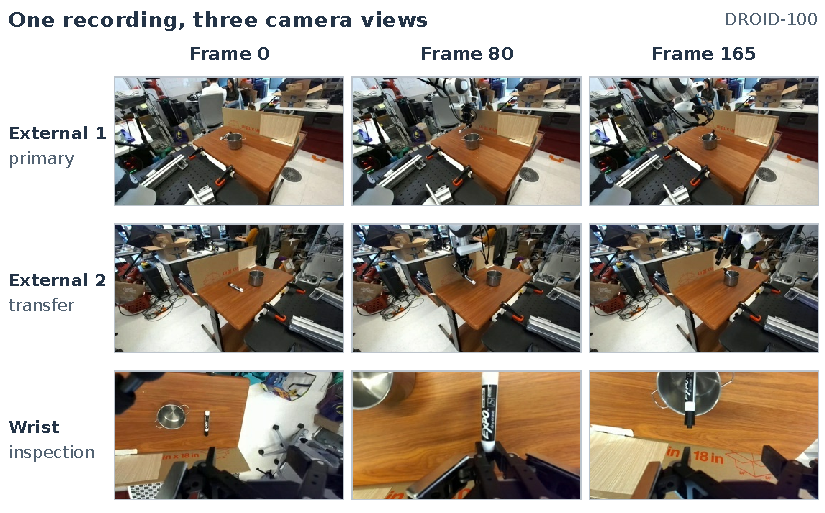
\includegraphics[width=\linewidth]{generated/real_video/recorded_droid_views.pdf}
\caption{\textbf{Actual recorded DROID camera views, shown for data inspection.}
Columns show native frame indices 0, 80 and 165 from the first decoded record
of the separately downloaded DROID-100 ingestion audit; rows show its two
external cameras and wrist camera. Selection uses evenly spaced frame positions,
not rewards or model outcomes. All frames retain their full field of view,
original colors and publisher-provided face blurring; no image is generated.
The row annotations describe the registered roles of these camera streams:
external camera 1 is the primary view, external camera 2 is reserved for
camera-transfer evaluation, and the wrist stream is retained for inspection.
The study itself uses 24 selected shards of the full DROID release, with
1,126 audited episodes, rather than this one-record ingestion example.
These are observations, not predicted images, successful-policy results or
an algorithm comparison. Native indices are not calibrated elapsed time.}
\label{fig:real-video-data}
\end{figure}

\paragraph{Data and splits.}
Before optimization, we fixed 24 of the full release's 2,048 shards by a salted
hash of their object names. This selection comprises 1,126 audited episodes
and 22,017,792,821 downloaded bytes including metadata and license.
Object generations, publisher checksums and local hashes identify the inputs.
We assign recording sessions, defined by site plus recording date, to
training, validation and test with fixed 70/15/15 hash thresholds. The resulting
splits contain 851, 143 and 132 episodes from 316, 59 and 58 disjoint sessions,
respectively, spanning 14 sites overall. All 327,498 native observations and
64,826 complete action blocks passed extraction and alignment checks.
Unparseable session identifiers fail the audit; there is no frame-level
fallback. Session separation does not guarantee distinct scenes or objects.
All recorded outcomes are retained without success-based selection.

\paragraph{Observation and action contract.}
Frames at native indices $0,5,10,\ldots$ are paired with the intervening five
seven-dimensional commands, concatenated into a 35-dimensional block.
The full extraction verified every native command array against the recorded
six Cartesian-position/pose components plus gripper position.
Incomplete tails are counted, and 11 episodes too short for an eight-frame
training window remain in the data. The inspected release has no per-step timestamp,
so horizons are expressed in native transitions. Ground-truth state, rewards,
success flags, language and future images are never context inputs.
Training and checkpoint selection use external camera 1 only; camera 2 on
held-out episodes provides a separately reported natural camera-transfer test.
No synthetic appearance corruption is applied in this study.

\paragraph{Representation and matched controls.}
We freeze DINOv2-small~\citep{oquab2023dinov2}, resize complete images to
$224\!\times\!224$, and pool the final patch grid into $2\!\times\!2$ spatial
cells, producing 1,536-dimensional targets. Feature and action normalization
is fitted on training camera 1 only. The pinned LeWM causal predictor
\citep{maes2026lewm} has width 192 and four transformer blocks; a residual
output head initializes every mode to persistence in the fixed feature space.
The four modes are Framewise, Constant dynamics, ShiftWM real-video variant
(ours), and an Action-free control. Each uses three training seeds and the
same common initialization, data and optimization: 12 registered runs, each
with 30 epochs. The model observes three support frames and recursively
predicts five further frames using recorded commands, without query-image
teacher forcing. We select checkpoints using validation forecast loss.

\paragraph{Evaluation and interpretation.}
We register horizons of 1, 3 and 5 action blocks, plus a separately labeled
10-block extrapolation test. Comparisons include persistence and constant
feature-velocity extrapolation, with raw and standardized feature MSE and
cosine error. We aggregate within episodes and quantify uncertainty by source
session and training seed. Camera-transfer and ordinary held-out results
remain separate. Reversing recorded query actions probes model sensitivity,
not the physical outcome of an unexecuted intervention. This observational
study provides neither paired canonical targets nor identified physical
factors; its metrics cannot establish closed-loop real-robot success.

\IfFileExists{tables/real_video_results.tex}{
\FloatBarrier
% Generated only after 12 complete runs, 48 validated evaluations, and portable-release verification.
\begin{table}[t]\centering\small
\setlength{\tabcolsep}{4pt}\renewcommand{\arraystretch}{1.12}
\begin{tabular}{lrrrr}\toprule
Method & MSE@1 $\downarrow$ & MSE@3 $\downarrow$ & MSE@5 $\downarrow$ & Gain@5 (\%) $\uparrow$\\\midrule
Framewise & $0.04988\pm2.2\!\times\!10^{-5}$ & $0.1031\pm4\!\times\!10^{-5}$ & $0.1385\pm0.00015$ & reference\\
Constant dynamics & $0.04987\pm2.2\!\times\!10^{-5}$ & $0.1031\pm5\!\times\!10^{-5}$ & $0.1384\pm0.00016$ & +0.04\\
\rowcolor{orange!9}
\textbf{ShiftWM (ours)} & $0.04979\pm4.2\!\times\!10^{-5}$ & $0.1029\pm0.00011$ & $0.1382\pm0.00011$ & \positivegain{+0.20}\\
Action-free & $0.04993\pm2.8\!\times\!10^{-5}$ & $0.1033\pm0.00011$ & $0.1389\pm0.00013$ & -0.28\\
\midrule
Persistence & $0.05029$ & $0.1053$ & $0.1424$ & -2.83\\
Constant velocity & $0.1207$ & $0.6215$ & $1.489$ & -975.22\\
\bottomrule\end{tabular}
\caption{\textbf{Recorded DROID: primary external-camera-1 forecasting.} Train-standardized feature MSE at 1, 3 and 5 action blocks (5, 15 and 25 native transitions); lower is better. Learned entries show three-seed mean $\pm$ sample SD; support-only baselines have no training-seed SD. Gain@5 is $100(\mathrm{Framewise}-\mathrm{method})/\mathrm{Framewise}$, a point reduction, not percentage points. \positivegain{Bold green} marks a positive point reduction, not significance. At five blocks, ours minus the named reference in MSE with 95\% paired session/seed bootstrap intervals is Framewise: $-0.0002808\;[-0.001038,0.000413]$ (includes zero); Constant dynamics: $-0.0002289\;[-0.0009871,0.0004498]$ (includes zero). Intervals are unadjusted for multiple comparisons; zero-crossing intervals are inconclusive.}
\label{tab:real-video-primary}\end{table}

\begin{table}[t]\centering\footnotesize
\setlength{\tabcolsep}{4pt}\renewcommand{\arraystretch}{1.12}
\begin{tabular}{lrrrr}\toprule
& \multicolumn{2}{c}{External camera 1} & \multicolumn{2}{c}{External camera 2}\\
\cmidrule(lr){2-3}\cmidrule(l){4-5}
Method & 5 blocks & 10 blocks & 5 blocks & 10 blocks\\\midrule
Framewise & $0.1385\pm0.00015$ & $0.1899\pm0.00085$ & $0.1543\pm8.9\!\times\!10^{-5}$ & $0.22\pm0.00066$\\
Constant dynamics & $0.1384\pm0.00016$ & $0.1898\pm0.00089$ & $0.1543\pm9.9\!\times\!10^{-5}$ & $0.2199\pm0.00066$\\
\rowcolor{orange!9}
\textbf{ShiftWM (ours)} & $0.1382\pm0.00011$ & $0.1935\pm0.004$ & $0.1542\pm0.00032$ & $0.2227\pm0.0031$\\
Action-free & $0.1389\pm0.00013$ & $0.1895\pm3.9\!\times\!10^{-5}$ & $0.1544\pm0.00016$ & $0.2188\pm0.00055$\\
\midrule
Persistence & $0.1424$ & $0.1937$ & $0.1574$ & $0.2214$\\
Constant velocity & $1.489$ & $5.114$ & $1.636$ & $5.637$\\
\bottomrule\end{tabular}
\caption{\textbf{Separate recorded-video populations.} Final-horizon standardized MSE; lower is better. External-camera-1/five-block is primary; camera 2 measures natural camera transfer, and ten blocks measure horizon extrapolation. The same session-disjoint test recordings are considered, but complete-window eligibility can differ by horizon. Three-seed means and sample SD are shown for learned methods. These feature forecasts do not measure closed-loop robot success. Raw MSE, cosine error, all paired intervals and reversed-action diagnostics are retained in the source-linked results report.}
\label{tab:real-video-transfer}\end{table}

}{}

\paragraph{Completed results.}
All 12 runs completed 30 epochs. On the primary camera, five-block
standardized feature MSE is 0.138198 for ShiftWM, 0.138479 for Framewise,
and 0.142392 for persistence. The 0.20\% reduction versus Framewise is
inconclusive: the paired 95\% MSE-difference interval is
$[-0.001038,0.000413]$. The 2.94\% reduction versus persistence has an
interval below zero, $[-0.006714,-0.001908]$; camera transfer retains a
2.02\% reduction versus persistence. At ten blocks, however, error is
1.91\% and 1.24\% higher than Framewise on the two cameras, respectively,
with both intervals including zero. These intervals are unadjusted for
multiple comparisons. Figure~\ref{fig:real-video-comparison} relates
recorded observations to the measured episode-level errors.

\paragraph{Training and action-use limitations.}
Every validation-selected checkpoint occurs at epoch 1 or 2; later
validation deterioration despite decreasing training loss indicates
overfitting. Reversing the order of future action blocks changes the
final-horizon error of ShiftWM by less than 0.10\% in every population.
This limited sensitivity is an observational diagnostic, not proof that
actions are unused or that physical interventions have no effect.
The completed study supports a modest short-horizon benefit over
persistence, while a substantial advantage over matched learned baselines
and reliable long-horizon action-dependent prediction remain unresolved.

\begin{figure}[p]
\centering
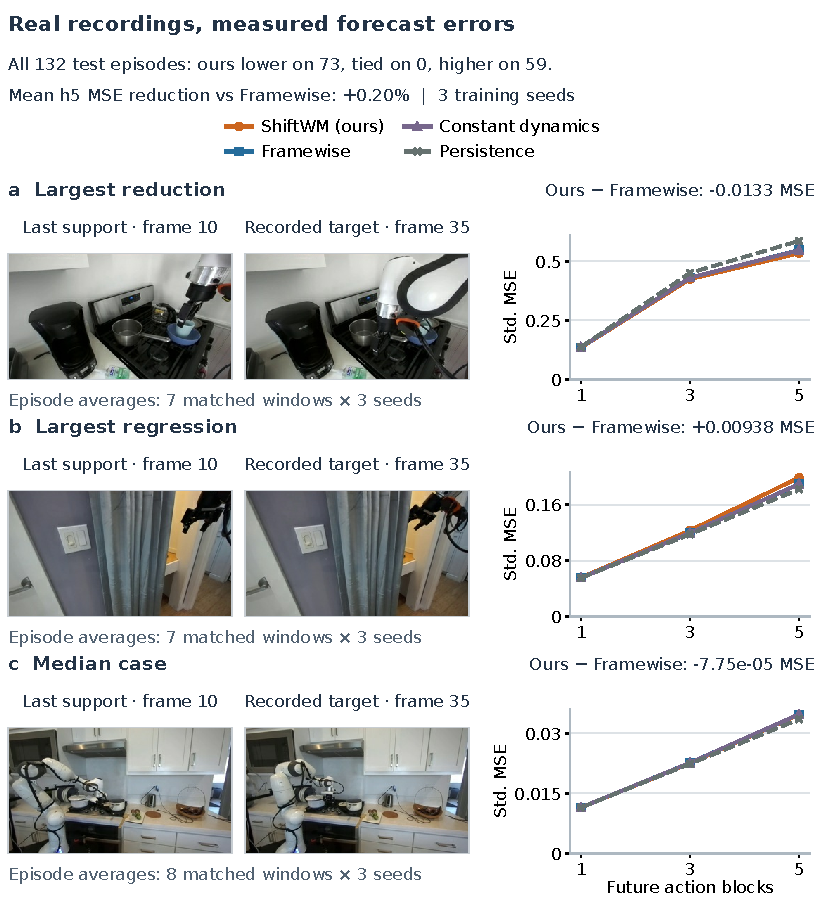
\includegraphics[width=\linewidth]{generated/real_video/comparison_recorded_droid.pdf}
\caption{\textbf{Real DROID recordings with measured feature-forecast errors.}
The primary held-out camera-1 population is summarized above three deterministically
selected episodes: the largest reduction, the largest regression, and an episode nearest the median in ours-minus-Framewise h5 standardized MSE
(ties by episode ID).
Each image pair shows the last observed support frame and final recorded query
target from the first evaluated window; these are actual photographs, not decoded
predictions. Each curve averages all evaluated windows of that episode, then all
three training seeds, at the three measured horizons. Panel y-axis ranges differ;
methods within each panel share the same axes. Curves show point means; the full-test paired 95\% h5 MSE-difference interval includes zero. The models observe three support
frames and recorded commands; persistence repeats the last support feature and
requires no training. The displayed images illustrate a recording and do
not localize the aggregate error or establish why a method wins. Selection is
outcome-conditioned and is not a frequency estimate: all-test counts and mean
reduction are reported above. Error reductions are feature-forecast differences,
not robot-control success or evidence of an identified causal mechanism.}
\label{fig:real-video-comparison}
\end{figure}


\subsection{Validation development: diagnosing and calibrating excess motion}
\label{app:real-video-calibration-development}
After completing the registered study, we investigated overfitting using
training and validation recordings only. Stronger command substitutions
clarify the reversal diagnostic: replacing future commands with a sequence
from another recording session increases the selected ShiftWM model's
ten-block validation error by 5.17\%, averaged across three seeds, whereas
the action-free control is unchanged. These are sensitivity probes against
the original recorded future, not outcomes of executed counterfactual actions.
Low-future-motion validation windows suffer relative to persistence, while
high-motion windows benefit; these target-defined strata are descriptive
and cannot determine an online adaptation rule.

We therefore evaluate a simple, matched residual-calibration control.
Let $r_h=\hat z_h-z_0$ denote the predicted displacement from the final
observed support feature and $d_h=z_h-z_0$ its recorded target, both in
the frozen training-standardized coordinates. For each selected checkpoint,
we fit a single scalar on training recordings:
\begin{equation}
 \alpha=\operatorname{clip}_{[0,1]}
 \frac{\mathbb{E}_{\mathrm{train}}\langle r_h,d_h\rangle}
      {\mathbb{E}_{\mathrm{train}}\|r_h\|_2^2},
 \qquad \tilde z_h=z_0+\alpha r_h .
 \label{eq:real-video-residual-calibration}
\end{equation}
We set $\alpha=0$ for zero predicted-displacement energy. The expectation
averages all ten horizons and feature dimensions, then windows within each
episode and equally across eligible training episodes. The base recursive
trajectory is unchanged; contraction is applied to its output.
All four methods and three seeds receive the same fitting procedure on
830 eligible training episodes and 7,721 windows; no new neural weights are
trained. The selected base checkpoints, data and scientific dependencies
remain frozen, and all twelve calibration configurations pass exact offline
CPU reload checks.

Table~\ref{tab:real-video-calibration-development} reports the complete
validation comparison. Calibration reduces our ten-block error by 1.66\%
relative to its own uncalibrated model. Against equally calibrated Framewise,
the reductions are 0.78\% at five blocks and 0.15\% at ten; the latter paired
interval includes zero. Both horizons use 141 eligible validation episodes
from 59 sessions, with 1,772 and 1,631 windows, respectively.
This standard least-squares control is development evidence, not a new
methodological contribution or a replacement for the original test results.
Any confirmatory evaluation of a revised method requires a separately
registered, untouched recording-session-disjoint population; its preparation
is pending and no results are claimed here.

% Generated from the completed full-training calibration campaign; VALIDATION ONLY.
\begin{table}[t]\centering\footnotesize
\setlength{\tabcolsep}{3.5pt}\renewcommand{\arraystretch}{1.12}
\begin{tabular}{lrrrrrr}\toprule
& \multicolumn{3}{c}{Validation: 5 blocks} & \multicolumn{3}{c}{Validation: 10 blocks}\\
\cmidrule(lr){2-4}\cmidrule(l){5-7}
Method & Original & Calibrated & Gain (\%) & Original & Calibrated & Gain (\%)\\\midrule
Framewise & 0.159071 & 0.158942 & \positivegain{+0.08} & 0.216903 & 0.216206 & \positivegain{+0.32}\\
Constant dynamics & 0.158998 & 0.158880 & \positivegain{+0.07} & 0.216746 & 0.216099 & \positivegain{+0.30}\\
\rowcolor{orange!9}
\textbf{ShiftWM (ours)} & 0.158398 & 0.157704 & \positivegain{+0.44} & 0.219507 & 0.215874 & \positivegain{+1.66}\\
Action-free & 0.159766 & 0.159718 & \positivegain{+0.03} & 0.217435 & 0.217144 & \positivegain{+0.13}\\
\bottomrule\end{tabular}
\caption{\textbf{Validation development: matched residual calibration, not a new test.} Train-standardized feature MSE, lower is better; all four methods and three seeds are included. One scalar per frozen best checkpoint is fitted on 830 eligible training episodes (7,721 windows), with no validation targets used for fitting. Each Gain column is the reduction from that row's own uncalibrated model. \positivegain{Bold green} marks positive point reductions, not significance. Against also-calibrated Framewise, ours improves 0.78\% at five blocks and 0.15\% at ten; the paired MSE differences with 95\% session/seed bootstrap intervals are $-0.001238\;[-0.002173,-0.000470]$ and $-0.000332\;[-0.001395,+0.001022]$, respectively. The latter includes zero. These are exploratory validation intervals, unadjusted for multiple comparisons; the original held-out results remain unchanged.}
\label{tab:real-video-calibration-development}\end{table}

